\documentclass{article}

% if you need to pass options to natbib, use, e.g.:
% \PassOptionsToPackage{numbers, compress}{natbib}
% before loading nips_2017
%
% to avoid loading the natbib package, add option nonatbib:
% \usepackage[nonatbib]{nips_2017}

%\usepackage{nips_2017}

% to compile a camera-ready version, add the [final] option, e.g.:
\usepackage[final]{nips_2017}

\usepackage[utf8]{inputenc} % allow utf-8 input
\usepackage[T1]{fontenc}    % use 8-bit T1 fonts
\usepackage{hyperref}       % hyperlinks
\usepackage{url}            % simple URL typesetting
\usepackage{booktabs}       % professional-quality tables
\usepackage{amsfonts}       % blackboard math symbols
\usepackage{nicefrac}       % compact symbols for 1/2, etc.
\usepackage{microtype}      % microtypography
\usepackage{wrapfig}
\usepackage{graphicx}
%\usepackage[demo]{graphicx}
\usepackage{caption}
\usepackage{subcaption}
\usepackage{float}
\title{Agricultural Commodity Price Analysis}

% The \author macro works with any number of authors. There are two
% commands used to separate the names and addresses of multiple
% authors: \And and \AND.
%
% Using \And between authors leaves it to LaTeX to determine where to
% break the lines. Using \AND forces a line break at that point. So,
% if LaTeX puts 3 of 4 authors names on the first line, and the last
% on the second line, try using \AND instead of \And before the third
% author name.

\author{
 Joseph Nunez\\
Mathematics of Big Data\\
Harvey Mudd College\\ 
May 30, 2018\\
jbnunez@hmc.edu}

\begin{document}
% \nipsfinalcopy is no longer used


\maketitle


\begin{abstract}
Internationally traded commodities' prices are impacted by a wide array of factors spread out around the world.  The United States Department of Agriculture puts together a monthly World Agricultural Supply and Demand Estimate (WASDE) report of a number of relevant variables for a number of agricultural commodities.  Combined with historical data on futures contracts for commodities, we apply multi-layer perceptrons, LSTMs, and PCA-augmented $k$-nearest neighbors to classify corn and soybean futures contract prices as going up or down in the near future.  We employ these methods on both the WASDE report data as well as historical futures contract prices to classify whether the futures price will increase or decrease in the near future.  While multi-layer perceptrons and LSTMs showed very poor performance, PCA-augmented $k$-nearest neighbors performed reasonably well on both market and WASDE data.  PCA-augmented $k$-nearest neighbors achieved 77.3\% accuracy on corn market data, 76.3\% accuracy on soybean market data, 80.9\% accuracy on corn WASDE data, and 76.5\% accuracy on soy WASDE data.

\end{abstract}




\section{Introduction}
Agricultural commodity prices are influenced by an extremely broad array of factors---trade regimes, international weather patterns, season, etc.  Fortunately, the USDA compiles a monthly report, called the World Agricultural Supply and Demand Estimate (WASDE).  For corn and soybeans, the WASDE report includes information on area planted, area harvested, yield, production, stocks, imports, and exports for the US, the world as a whole, and other countries and regions responsible for significant production.  In total, the corn section of the report contains 112 variables and the soybean section contains 69 variables.  The difference largely arises from there being more countries and regions included in the corn report and the fact that corn is an input to ethanol, and demand is therefore impacted by the price of oil.
Combined with market data for commodity futures contracts from an exchange (obtained through Quandl.com), these data points were used as features with which to explore classification techniques.  We attempted multilayer perceptrons (MLP), long short-term memory networks (LSTM), and PCA-augmented $k$-nearest neighbors.
We labeled the data by looking at the daily close price of futures contracts for corn and soybeans and determining whether that value increased or not.  As features, we used both the economic data from the WASDE report and the recent historical data from the futures contract.    

Multi-layer perceptrons simply refer to feed-forward neural networks with densely connected layers, and are commonly used for regression problems.  
Long short-term memory networks are recurrent neural networks which incorporate a memory state that allows the network to distinguish between instances which occurred recently from those which occurred longer ago.  
As such these networks are frequently employed in tackling time-series regression problems.  
Principal component analysis identifies a set of orthogonal axes along which the greatest variation occurs, and allows the data to be represented in a lower dimension and in such a way that principal components are generally unrelated.  This representation allows the $k$-nearest neighbors algorithm (which classifies samples by a plurality vote of the points nearest them) to identify neighbors based on the components of greatest variation, since less significant components will have very little difference between points.




\section{Methods}
%\begin{wrapfigure}{r}{0.3\textwidth}
%\includegraphics[scale=0.2]{simplex}
%\caption{A simplex in R3 [8]}
%\end{wrapfigure}
We used two different types of features for classification: constructing the feature vector from market data and from economic data. 
For all data points, the values were normalized to all be between 0 and 1 by subtracting by the minimum across all data in that field, then dividing by the difference between minimum and maximum.  
For both data sets, I used the prices from the market data to determine whether the price of the given commodity (corn or soybeans) went up or down in a given time step. 
If the price increases over the following time period---one month for economic data and one trading day for market data---that data point was labeled true; otherwise, it was labeled false.  
For the MLP and LSTM labels, the label was simply the normalized price.
For the economic data, the feature vector was simply all of the entries provided in the WASDE report.
For the market data, the feature vector consisted of open, high, low, close, volume, and open interest for each of the previous $d$ trading days, where $d$ ranged from 0 to 22 (22 trading days being approximately one month).
We then ran PCA with both two and three principal components in Python using scikit-learn and visualized the results using matplotlib in order to see whether the data are separable by label.  Since no differences in separation could be observed for different values of $d$, we arbitrarily chose to proceed by using $d=22$.
To construct training and test sets, we set aside 20\% of the data for testing, while the other 80\% was used for training.

After observing that the labels began to show some separation under PCA with very few components, we employed PCA with higher numbers of components then used a $k$-nearest neighbors classifier to label the data based on this.  
We attempted all values of $k$ from 2 to 30 and all numbers of principal components from 2 to 40 (higher values of $k$ and numbers of components are not displayed in the results section because they did not lead to improved accuracy.  

The MLP was used for the WASDE data sets, and consisted of 5 layers: an input layer of the size of the input data, a 256 neuron layer, another 256 neuron layer, a 32 neuron layer, and a 1 neuron output layer, where the output layer uses a sigmoid activation function and all previous layers use a linear activation function.  The layer sizes and activation functions were empirically determined by testing layer sizes of 2 to 256 (in powers of 2) in succession until the error began to flatline.  The error we used as the mean square error.  The network was trained using the Adam optimizer with a decay rate of 0.4.  

The LSTM was used for the futures market data sets, and consisted of 5 layers: an input layer of the size of the input data, a 256 neuron LSTM layer, another 256 neuron LSTM layer, a 32 neuron dense layer, and a 1 neuron output layer, where the output layer uses a sigmoid activation function and the dense layer uses a relu activation function.  As before, the layer sizes and activation functions were empirically determined, the error used was mean square error, and the network was trained using the Adam optimizer with a decay rate of 0.4.  Both the LSTM and the MLP were implemented using the Keras package in python.

We then want to find the accuracy of the MLPs and LSTMs in predicting market direction in a way comparable to our PCA-KNN classifier, so rather than use mean square error, we will evaluate the accuracy in terms of correctly predicting direction.  To do so, for each sample, if the target and predicted prices are both above or both below the most recent price, then that prediction is marked correct.  Otherwise, the prediction is marked incorrect.  This is the metric which will be used to describe accuracy of the neural network models in the results.


\section{Results}
First, observe the results of running PCA with 2 principal components using the USDA WASDE report data as our feature vectors.

\begin{figure}[h!]
\centering
\begin{subfigure}{.5\textwidth}
  \centering
  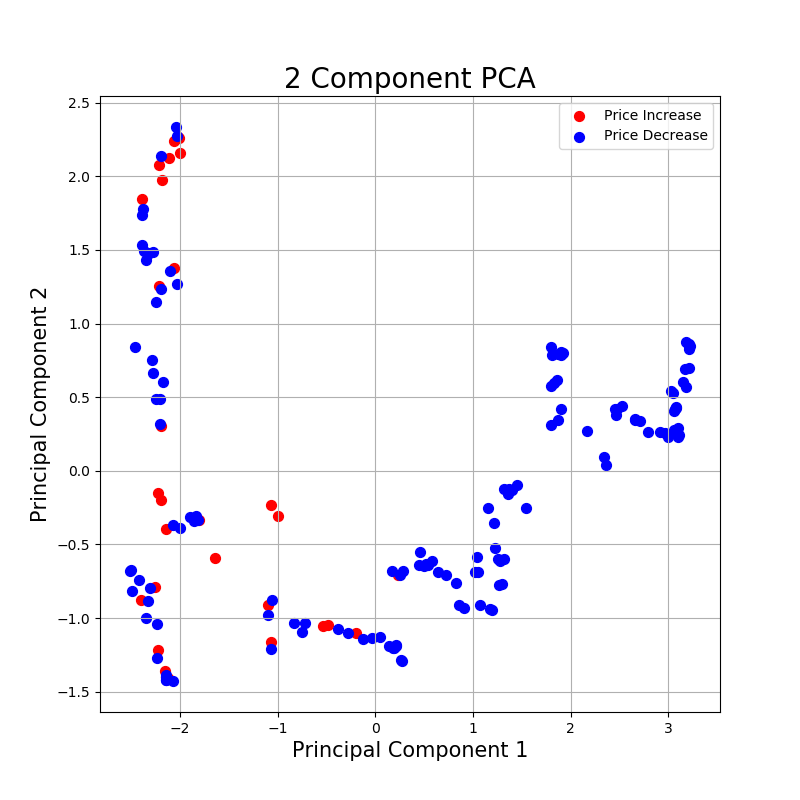
\includegraphics[scale=.3]{imagesmid/fullcorn}
\caption{Corn}
\end{subfigure}%
\begin{subfigure}{.5\textwidth}
  \centering
  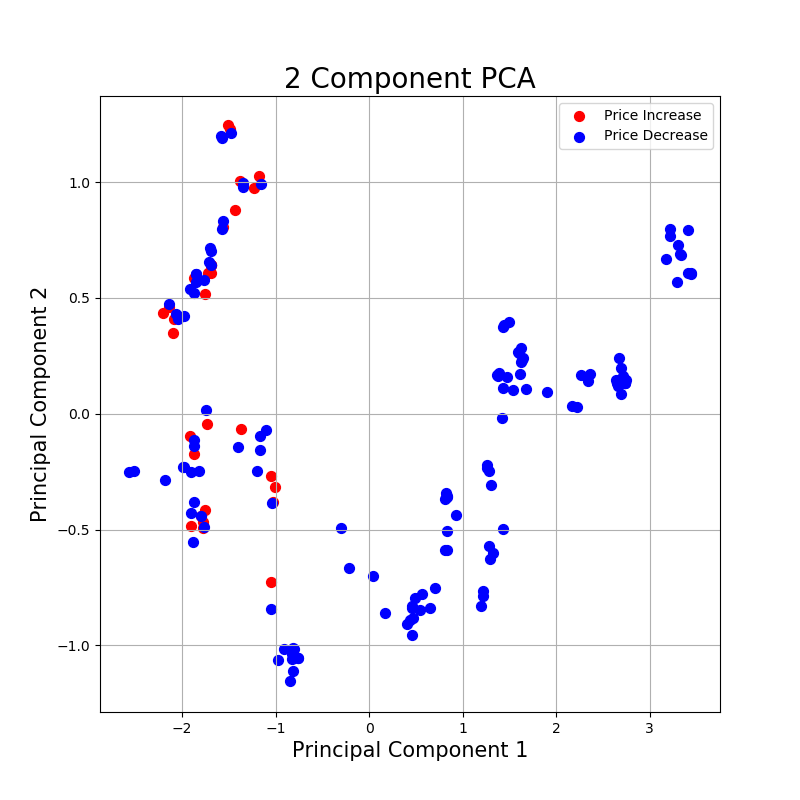
\includegraphics[scale=.3]{imagesmid/fullsoy}
\caption{Soybean}
\end{subfigure}
\caption{WASDE data with 2 components}
\end{figure}

As we can see, for both corn and soybeans, the data does not become cleanly separated into increasing and decreasing prices, but there is some separation of a group of points which all lead to decreasing prices.  This is still a useful finding, as we can use this information to predict that the price will fall if a WASDE report produces a point in the cluster which consistently sees a price decrease.  Next, observe the 3 component PCA results:

\begin{figure}[h!]
\centering
\begin{subfigure}{.5\textwidth}
  \centering
  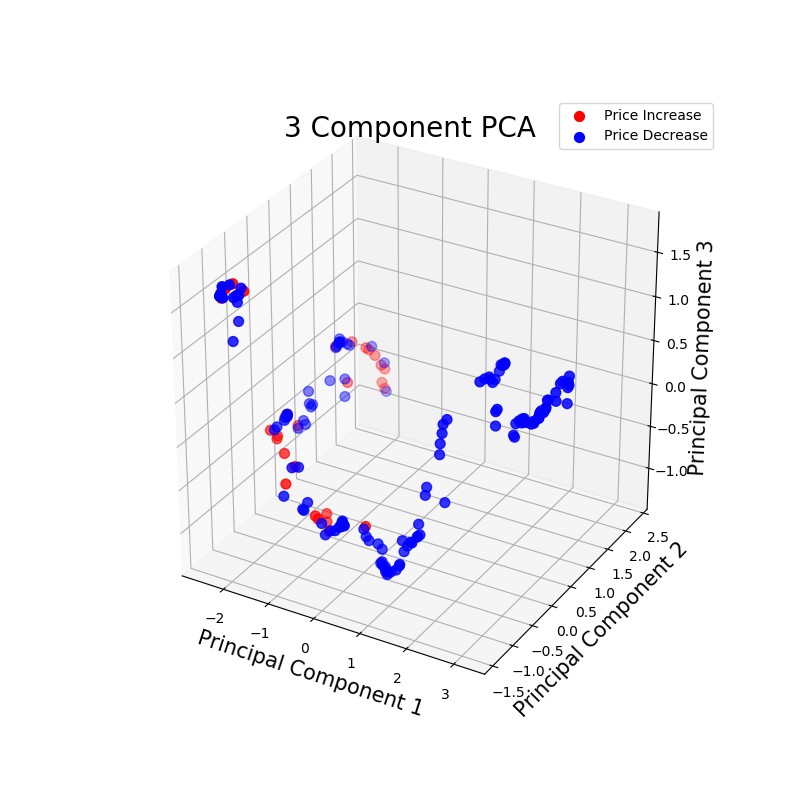
\includegraphics[scale=.4]{imagesmid/fullcorn3d}
\caption{Corn}
\end{subfigure}%
\begin{subfigure}{.5\textwidth}
  \centering
  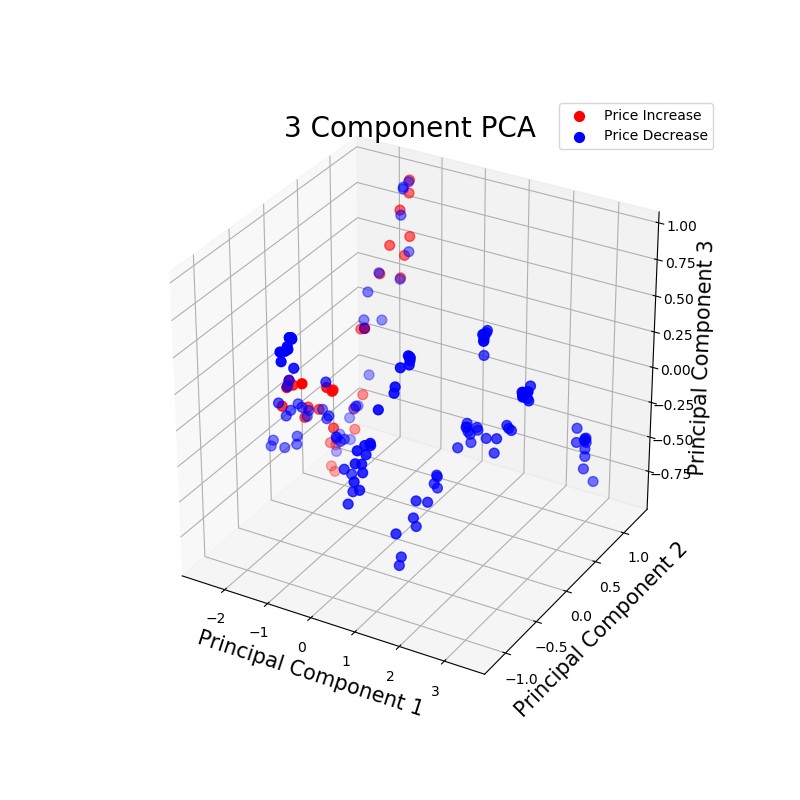
\includegraphics[scale=.4]{imagesmid/fullsoy3d}
\caption{Soybean}
\end{subfigure}
\caption{WASDE data with 3 components}
\end{figure}

Unfortunately, adding a third principal axis produced little additional separation, as the points for increasing and decreasing price in the left cluster are still thoroughly intermingled.

Next, we look at the PCA results for the market data for futures contracts, where $k$ is the number of previous days (not counting the current day) of market data used to predict the price movement in the following day.

\begin{figure}[h!]
\centering
\begin{subfigure}{.5\textwidth}
  \centering
  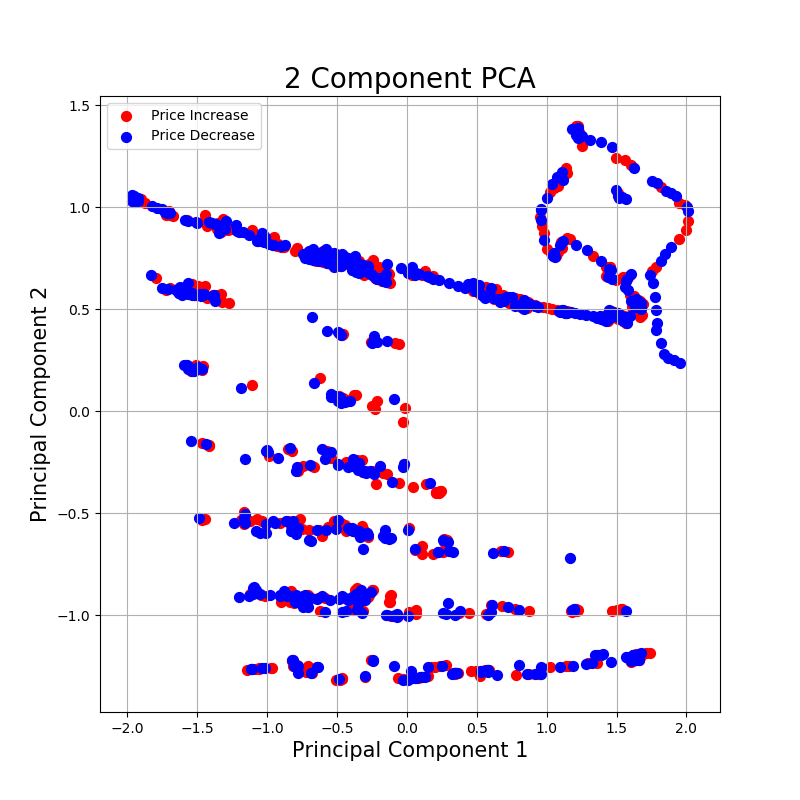
\includegraphics[scale=.3]{imagesmid/cornmkt5}
\caption{Corn}
\end{subfigure}%
\begin{subfigure}{.5\textwidth}
  \centering
  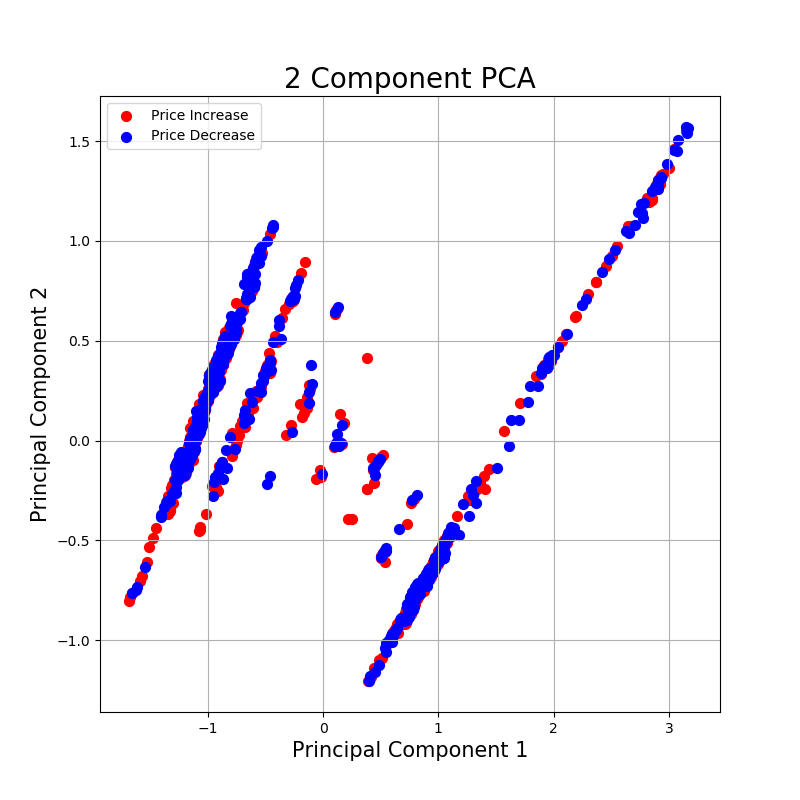
\includegraphics[scale=.3]{imagesmid/soymkt5}
\caption{Soybean}
\end{subfigure}
\caption{Futures data with 2 components and $d=5$}
\end{figure}

As we can see, there is no visible separation between rising and lowering prices when two principal components are used.  More values of $d$ were also used, but all showed a similar lack of separation, and the images are attached.  Next, observe the results of PCA with 3 components on the futures market data.  

\begin{figure}[h!]
\centering
\begin{subfigure}{.5\textwidth}
  \centering
  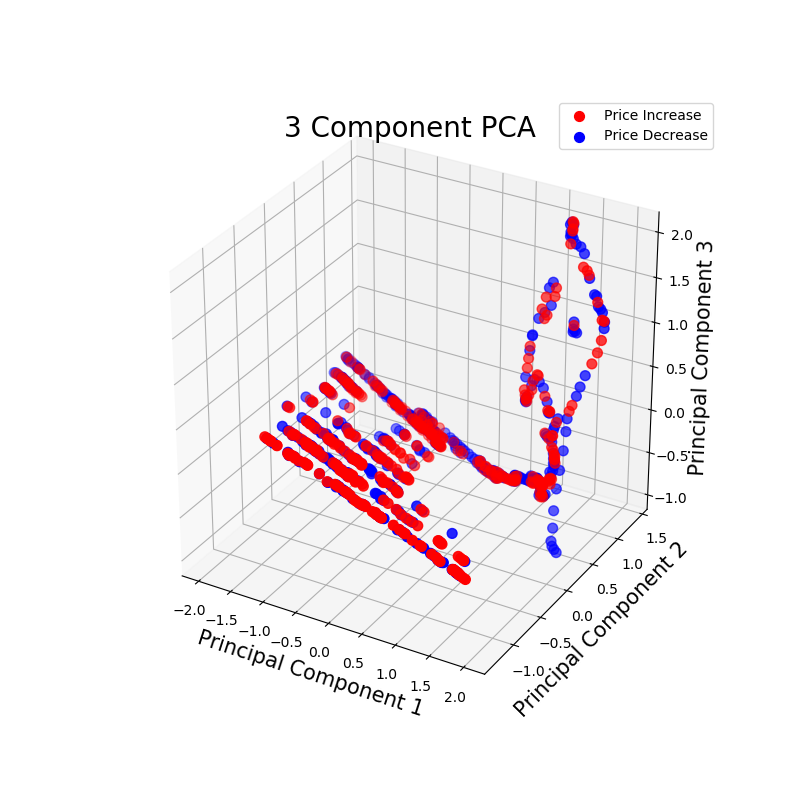
\includegraphics[scale=.4]{imagesmid/cornmkt5,3d}
\caption{Corn}
\end{subfigure}%
\begin{subfigure}{.5\textwidth}
  \centering
  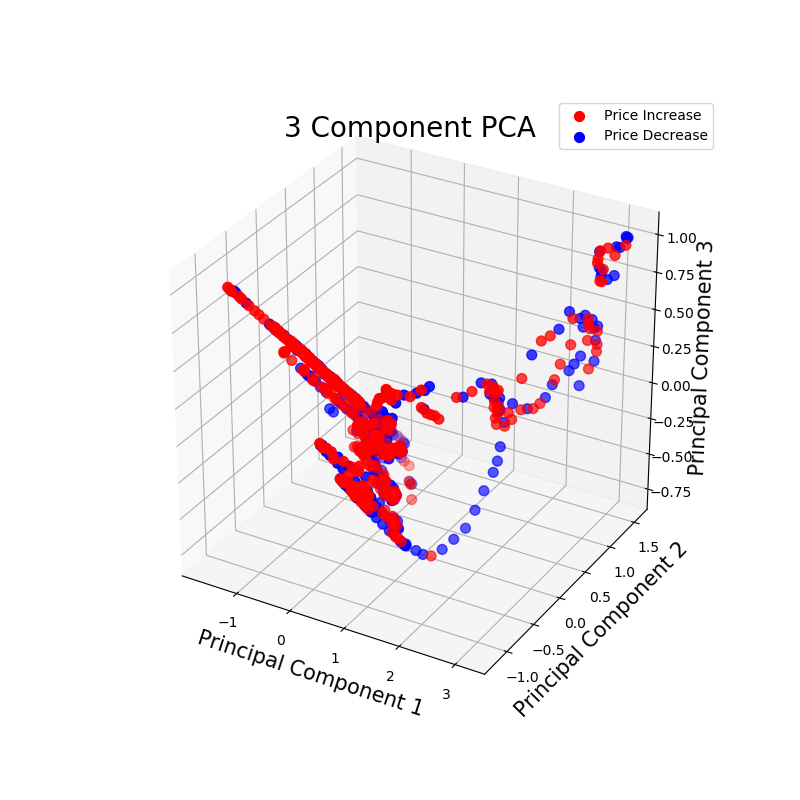
\includegraphics[scale=.4]{imagesmid/soymkt5,3d}
\caption{Soybean}
\end{subfigure}
\caption{Futures data with 3 components and $d=5$}
\end{figure}

Under three principal components, the data still appears largely unseparated.  However, as we can somewhat see in Figure 5, the points with increasing price lie very slightly ``above'' (in terms of the third component) the price decrease points which have similar locations in the first two components.  

A useful benchmark for evaluating classification models is the most frequent label benchmark, i.e. what percentage of guesses would be correct if you always predicted the label which appears most frequently.  For my testing sets, the most frequent labels were
\begin{center}
\begin{tabular}{|c|c|c|}
\hline
Dataset & Most Frequent Label & Frequency\\
\hline
Corn WASDE & Down & 52.17\%\\
Corn Market & Up & 51.98\%\\
Soybean WASDE & Up & 52.17\%\\
Soybean Market & Up & 53.83\%\\
\hline
\end{tabular}
\end{center}
Note that the rates are different for WASDE data and market data because the market data was used to predict daily shifts while the WASDE data was used for one week shifts and was only collected monthly.


The MLP and LSTM-based classifiers produced quite poor accuracy, as seen in the table below.
\begin{center}
\begin{tabular}{|c|c|}
\hline
Dataset & Accuracy\\
\hline
Corn WASDE & 61.3\%\\
Corn Market & 49.9\%\\
Soybean WASDE & 54.8\%\\
Soybean Market & 51.2\%\\
\hline
\end{tabular}
\end{center}

Only the MLP-based Corn WASDE data classifier meaningfully outperformed the most frequent label benchmark, but even then by a fairly small amount.  Interestingly, it outperformed the Soybean WASDE data, indicating that either the extra length of the WASDE data (112 points versus 69 points) had significant predictive value, or that Soybean prices are simply less predictable than corn.  The LSTM classifiers were both less accurate than the most frequent label.  The predicted prices versus actual prices for the MLP and LSTM are displayed below.

\begin{figure}[H]
\centering
\begin{subfigure}{.5\textwidth}
  \centering
  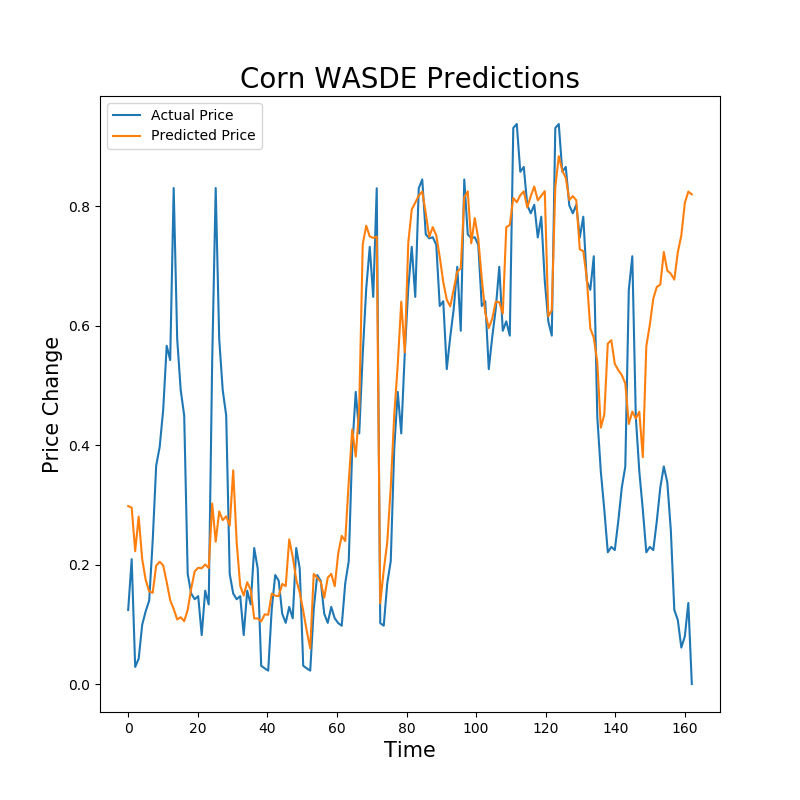
\includegraphics[scale=.38]{images/CornWASDE}
\caption{Corn}
\end{subfigure}%
\begin{subfigure}{.5\textwidth}
  \centering
  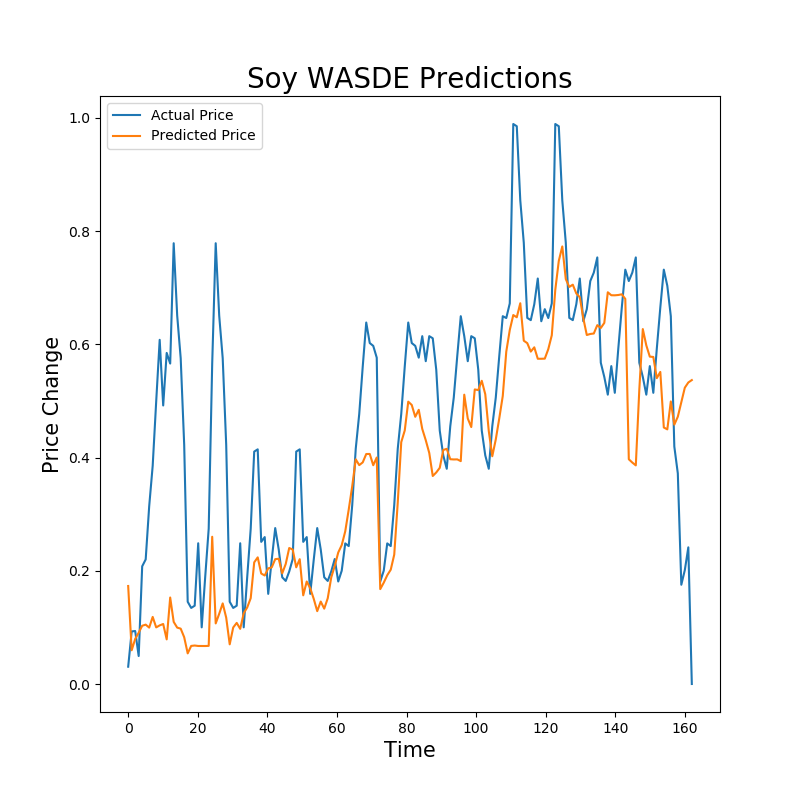
\includegraphics[scale=.38]{images/SoyWASDE}
\caption{Soybeans}
\end{subfigure}
\caption{MLP WASDE Data Classification}
\end{figure}

\vfill

\begin{figure}[H]
\centering
\begin{subfigure}{.5\textwidth}
  \centering
  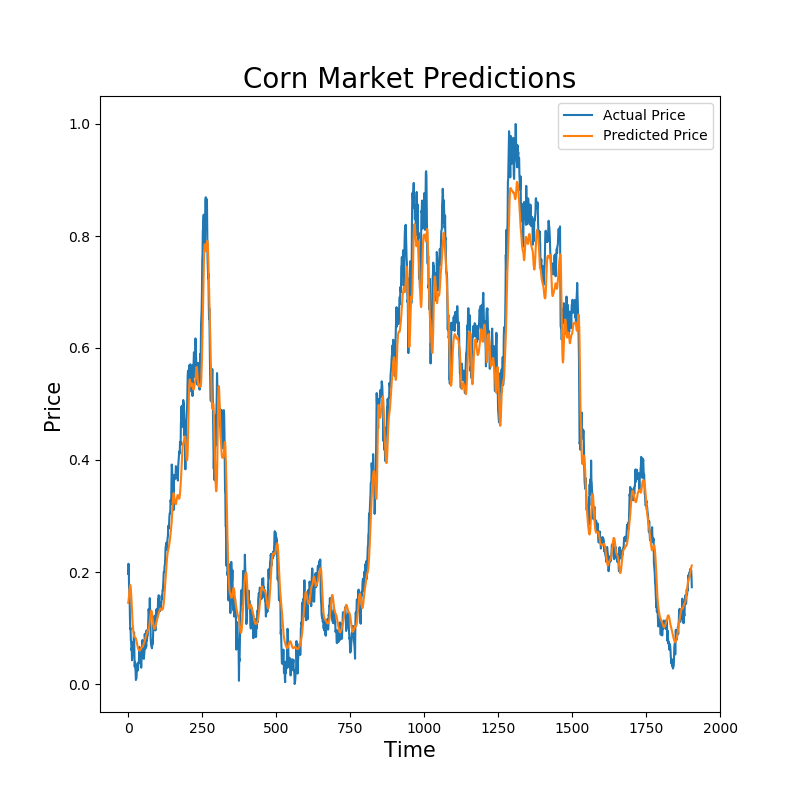
\includegraphics[scale=.38]{images/CornMarket}
\caption{Corn}
\end{subfigure}%
\begin{subfigure}{.5\textwidth}
  \centering
  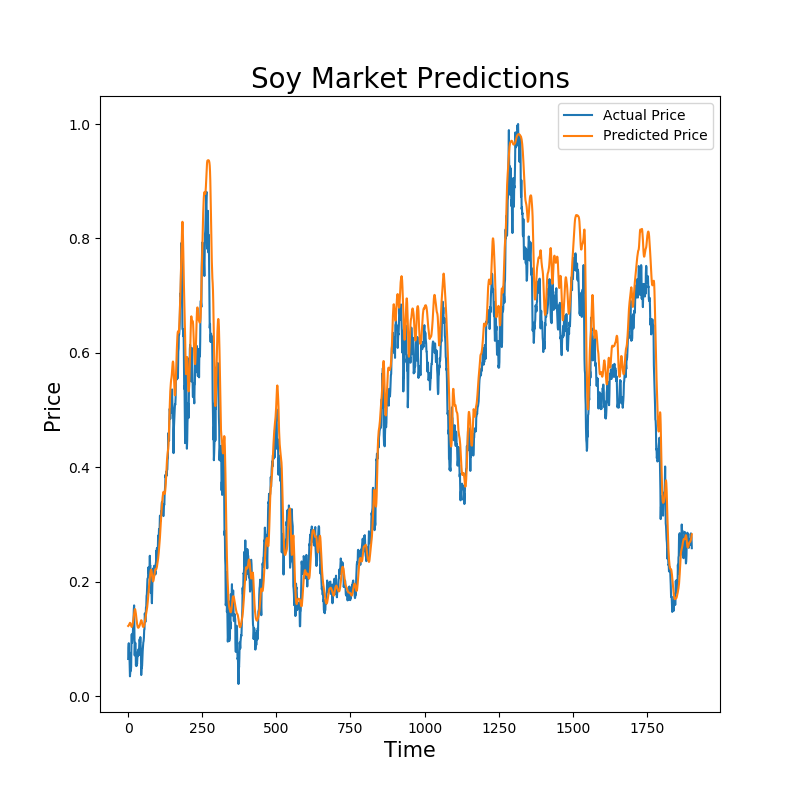
\includegraphics[scale=.38]{images/SoyMarket}
\caption{Soybeans}
\end{subfigure}
\caption{LSTM Market Data Classification}
\end{figure}

Interestingly, despite the LSTM predictions appearing to more closely track the actual prices than the MLP predictions, they are actually worse at guessing the direction.  A closer look at the LSTM prediction curve reveals that the LSTM was essentially just guessing the most recent price.

Note that though higher values of $k$ and both higher and lower numbers of components were tested, they never produced higher accuracy, so only the relevant plot is displayed\footnote{Other plots are included in the submission.}.

\begin{figure}[H]
\centering
\begin{subfigure}{.5\textwidth}
  \centering
  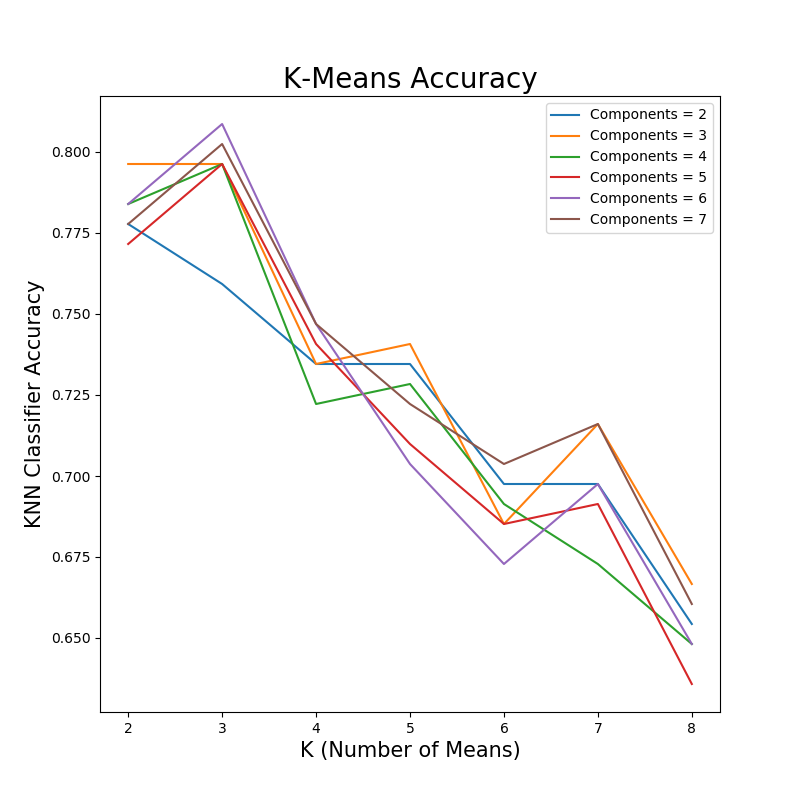
\includegraphics[scale=.38]{images/cornacc2,7,w}
\caption{Corn}
\end{subfigure}%
\begin{subfigure}{.5\textwidth}
  \centering
  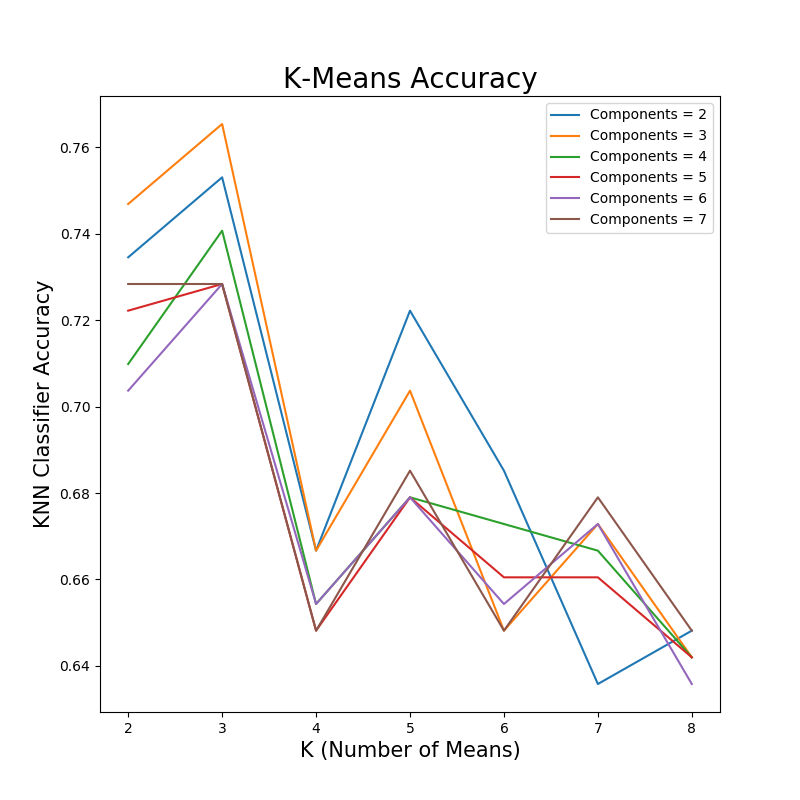
\includegraphics[scale=.38]{images/soyacc2,7,w}
\caption{Soybeans}
\end{subfigure}
\caption{PCA-KNN WASDE Data Classification}
\end{figure}


\begin{figure}[H]
\centering
\begin{subfigure}{.5\textwidth}
  \centering
  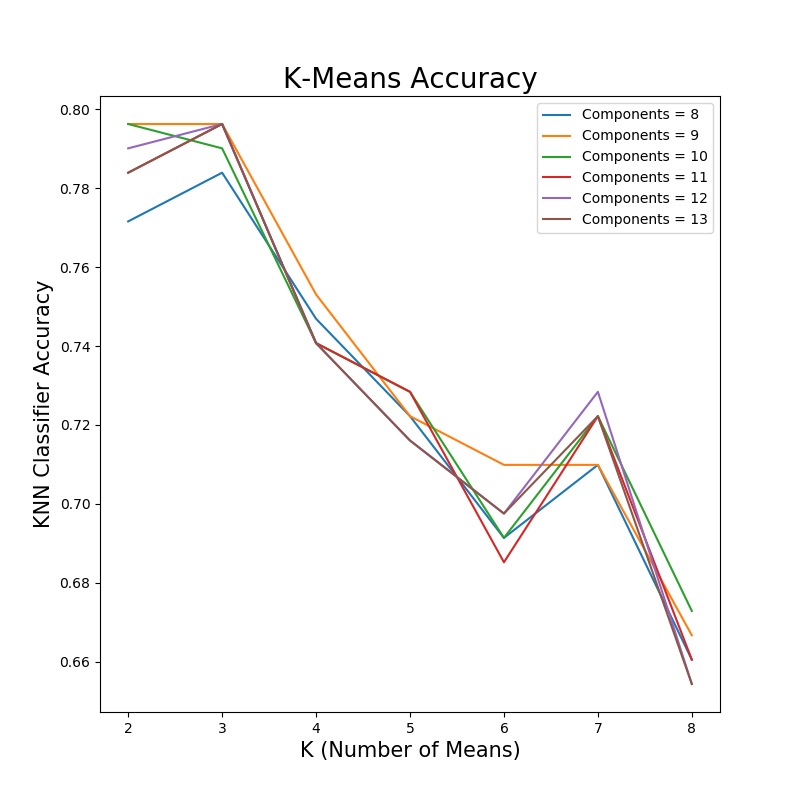
\includegraphics[scale=.38]{images/cornacc8,13,m}
\caption{Corn}
\end{subfigure}%
\begin{subfigure}{.5\textwidth}
  \centering
  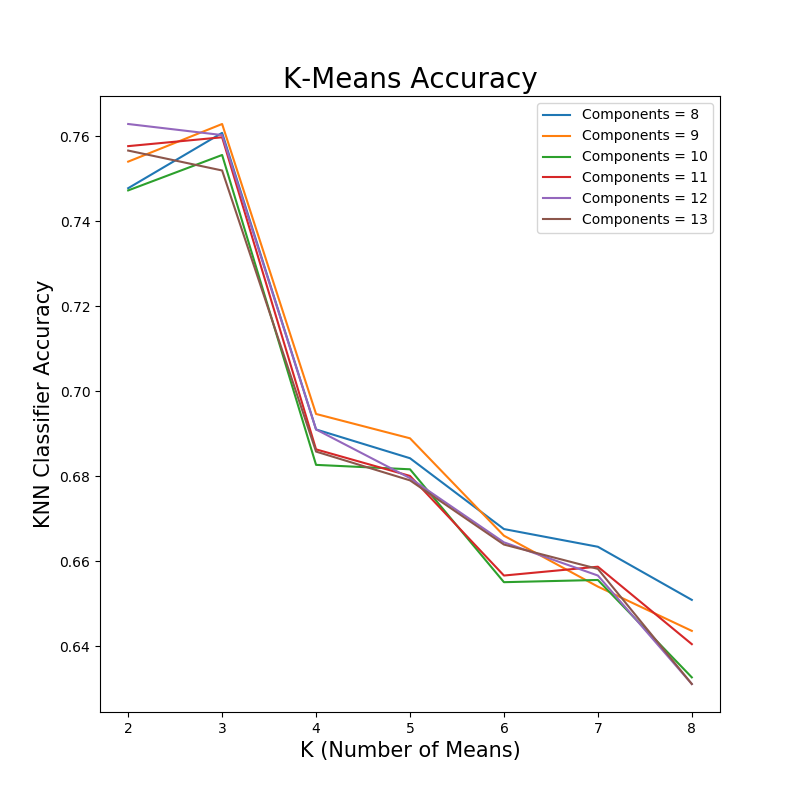
\includegraphics[scale=.38]{images/soyacc8,13,m}
\caption{Soybeans}
\end{subfigure}
\caption{PCA-KNN Market Data Classification}
\end{figure}



As seen in the graphs and in the table below, the best performance consistently occurred with $k=3$ neighbors.  

\begin{center}
\begin{tabular}{|c|c|c|c|}
\hline
Dataset & $k$ & Components & Accuracy\\
\hline
Corn WASDE & 3 & 6 & 80.9\%\\
Corn Market & 3 & 8 & 77.3\%\\
Soybean WASDE & 3 & 3 & 76.5\%\\
Soybean Market & 3 & 9 & 76.3\%\\
\hline
\end{tabular}
\end{center}

This performance is noticeably better than our most frequent labor benchmark and the performance of our MLP and LSTM classifiers.  
Interestingly, the soybean WASDE data classifier did not outperform the soybean market data classifier, while the corn WASDE data classifier did outperform its market counterpart.  This pattern mirrors the improved performance of the corn WASDE MLP-based classifier.  


\section{Conclusions}
Neural network-based approaches produced lackluster results which were essentially coin tosses.  
The only one which showed significant improvement was the MLP-based corn WASDE classifier, which showed slightly improved but nonetheless unimpressive performance, suggesting that the corn WASDE report is particularly insightful.  

The PCA-augmented $k$-nearest neighbors classifiers performed significantly better, all getting accuracies in the 76-81\% range.  While these accuracies are by no means overwhelming, for financial markets, this certainly appears to be accurate enough to use to implement a reliable trading strategy.  Assuming that the misclassified price changes are of similar magnitude to the correctly classified shifts, we would expect the return rate of such a strategy to be around half of the sum of the absolute values of all the price changes for each interval.  

The different number of components which proved optimal for different data sets is interesting.  The greater number of components in corn versus soybean WASDE data can be explained by the greater number of factors included in the corn WASDE report.  The greater number of components in the soybean versus corn market data may be a consequence of the fact that soybean prices have been consistently harder to classify than corn prices, so the extra dimension may be necessary to make better decisions.


\section{Future Work}
It is possible that day-long time intervals between market data samples are too long for an LSTM to be able to extract meaningful trends.  Markets may simply be too volatile over the course of single day for daily data to provide significant information.  It is possible that incorporating intraday pricing will improve performance, so studying the viability of intraday trading models could be a fruitful next step.  Additionally, it would be interesting to determine whether the PCA-KNN approach transfers to a shorter time frame.

It is also likely that a more sophisticated neural network should be able to provide accuracy in the 80\% range.  In particular, softmax activation functions coupled with convolutional layers may provide comparable performance to PCA-KNN, since convolutional layers have been proved to be equivalent to PCA and softmax may provide a similar categorization effect to KNN.  However, such an approach would essentially just be reproducing the effect of PCA-KNN, rather than creating a novel approach.  

Another avenue would be to use a composite approach which utilizes both market and WASDE data to make classifications, though such an approach is made difficult by the different frequencies with which both sets of data are available.

\section*{References}

[1] Murphy, Kevin, \textit{Machine Learning:
A Probabilistic Perspective}, Cambride, MA: Massachusetts Institute of Technology, 2012. \textit{Web}.

[2] Galarnyk, Michael, `Principle Component Analysis (PCA) for Data Visualization'
, Github.org, \url{https://github.com/mGalarnyk/Python_Tutorials/blob/master/Sklearn/PCA/PCA_Data_Visualization_Iris_Dataset_Blog.ipynb}

[3] Chen, Kai, Yi Zhou, and Fangyan Dai, `A LSTM-based method for stock returns prediction: A case study of China stock market,' IEEExplore, 2015, \url{https://ieeexplore.ieee.org/stamp/stamp.jsp?arnumber=7364089}

Data Sources:

[3] `Corn \& Soybean Prices 2008-2017', Kaggle, \url{https://www.kaggle.com/ainslie/usda-wasde-monthly-corn-soybean-projections}

[4] Quandl, \url{quandl.com}

\end{document}
